\begin{figure}[tbp]
  \centering
  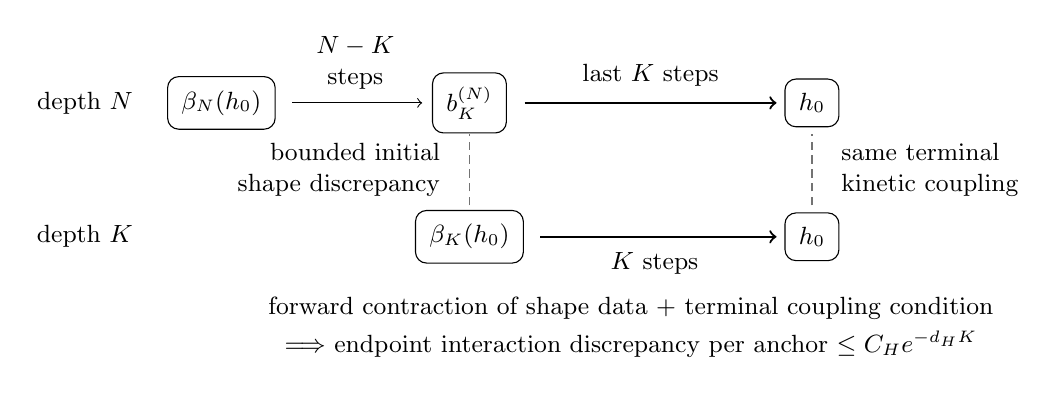
\begin{tikzpicture}[x=1cm,y=1cm,font=\small]
    \node[anchor=east] at (0,1.7) {depth $N$};
    \node[draw,rounded corners,inner sep=5pt] at (1.0,1.7)
      {$\beta_N(h_0)$};
    \draw[->] (1.9,1.7) -- (3.55,1.7);
    \node[above,align=center] at (2.7,1.75) {$N-K$\\steps};
    \node[draw,rounded corners,inner sep=5pt] at (4.15,1.7)
      {$b_K^{(N)}$};
    \draw[->,thick] (4.85,1.7) -- (8.05,1.7);
    \node[above] at (6.45,1.78) {last $K$ steps};
    \node[draw,rounded corners,inner sep=5pt] at (8.5,1.7) {$h_0$};

    \node[anchor=east] at (0,0) {depth $K$};
    \node[draw,rounded corners,inner sep=5pt] at (4.15,0)
      {$\beta_K(h_0)$};
    \draw[->,thick] (5.05,0) -- (8.05,0);
    \node[below] at (6.5,-0.08) {$K$ steps};
    \node[draw,rounded corners,inner sep=5pt] at (8.5,0) {$h_0$};

    \draw[densely dashed,black!55] (4.15,0.4) -- (4.15,1.3);
    \node[anchor=east,align=right] at (3.9,0.85)
      {bounded initial\\shape discrepancy};
    \draw[densely dashed,black!55] (8.5,0.4) -- (8.5,1.3);
    \node[anchor=west,align=left] at (8.75,0.85)
      {same terminal\\kinetic coupling};

    \node[align=center] at (6.2,-1.15)
      {forward contraction of shape data + terminal coupling condition\\[3pt]
       $\Longrightarrow$ endpoint interaction discrepancy per anchor $\le C_H e^{-d_H K}$};
  \end{tikzpicture}\par\medskip
  \caption{The comparison aligns the last $K$ blocking steps of two
  admitted trajectories with $N\ge K$. Here $b_K^{(N)}$ is the longer
  trajectory's coupling after its first $N-K$ steps. Their kinetic couplings agree
  at the terminal scale. Their complete endpoint laws need not agree:
  contraction bounds the discrepancy in their local interaction data,
  while bulk scalars are tracked separately. The bound is uniform in
  the number $N-K$ of earlier steps.}
  \label{fig:matched-trajectories}
\end{figure}
